\usepackage{listings}
\usepackage{xcolor}

% Define a custom style for VHDL
\lstdefinelanguage{VHDL}{
    keywords=[1]{library, use, entity, is, port, in, out, architecture, of, begin, end, process},
    keywords=[2]{signal, STD_LOGIC, STD_LOGIC_VECTOR},
    keywordstyle=[1]\color{blue}\bfseries,
    keywordstyle=[2]\color{teal}\bfseries,
    sensitive=true,
    morecomment=[l]--,
    morestring=[b]"
}

\lstset{
    language=VHDL,
    basicstyle=\ttfamily\footnotesize,
    numbers=left,
    numberstyle=\tiny\color{gray},
    keywordstyle=\color{blue},
    commentstyle=\color{green!60!black},
    stringstyle=\color{orange},
    breaklines=true,
    showstringspaces=false,
    tabsize=2,
    xleftmargin=2em
}

\begin{document}

\begin{Large}
    \textsf{\textbf{Carry Select Adder a 16 bit}}\\
\end{Large}
\textbf{Relazione di progetto}

\vspace{1ex}

\textsf{\textbf{Studenti:}} \\
\text{Frega Umberto 239527}, \href{frgmrt04a05l353d@studenti.unical.it}{\texttt{frgmrt04a05l353d@studenti.unical.it}};\\
\text{Napoli Leonardo 234364}, \href{npllrd02s30d086@studenti.unical.it} {\texttt{npllrd02s30d086@studenti.unical.it}};

\href{https://github.com/Zi0LEO/elettronica_digitale}{\texttt{Codice Sorgente}}


\vspace{2ex}

Il progetto assegnato consiste nel progettare ed implementare un carry select adder a 16 bit tramite linguaggio VHDL.
Per la progettazione del sistema si è deciso di utilizzare un pattern comportamentale, andando quindi a definire il comportamento del sistema in base a determinate condizioni, oltretutto si è optato per l'utilizzo del tipo \textit{STD\_LOGIC} e quindi \textit{STD\_LOGIC\_VECTOR} per una maggiore flessibilità e maggiori funzionalità.

Il primo passo della progettazione è stato definire la modularizzazione dell'adder tramite adder più semplici a minori bit. 
A questo riguardo si è optato per utilizzare 4 ripplecarry adder a 4 bit, ognuno formato da 4 full-adder.

\section{Full-Adder}
\subsection{Implementazione}
Come componente di base del sistema si è optato per un semplice full-adder. A causa della decisione di approcciare il problema in maniera comportamentale piuttosto che strutturale già nel caso base possiamo vedere l'utilizzo di un assegnamento della variabile \textit{carry\_out} tramite condizioni.

\begin{problem}{Codice Full-Adder}{problem-label}
\begin{lstlisting}[language=VHDL]
library IEEE;
use IEEE.STD_LOGIC_1164.ALL;

entity fulladder_1bit is
  Port ( 
    A : in STD_LOGIC;
    B : in STD_LOGIC;
    carry_in : in STD_LOGIC;
    carry_out : out STD_LOGIC;
    sum : out STD_LOGIC);
end fulladder_1bit;

architecture Behavioral of fulladder_1bit is
  signal p: STD_LOGIC;
begin
  p <= A xor B;
  carry_out <= A when p='0' else
    carry_in when p='1' else 'X';
  sum <= p xor carry_in;

end Behavioral;

\end{lstlisting}
\end{problem}
\newpage
\subsection{Schematica}
Il codice precedente ha generato in Vivado la schematica riportata in \textit{Figure 1}. Da notare la creazione di RTL\_MUX causata dal blocco condizionale \textit{when else};

\begin{figure}[h]
    \centering
    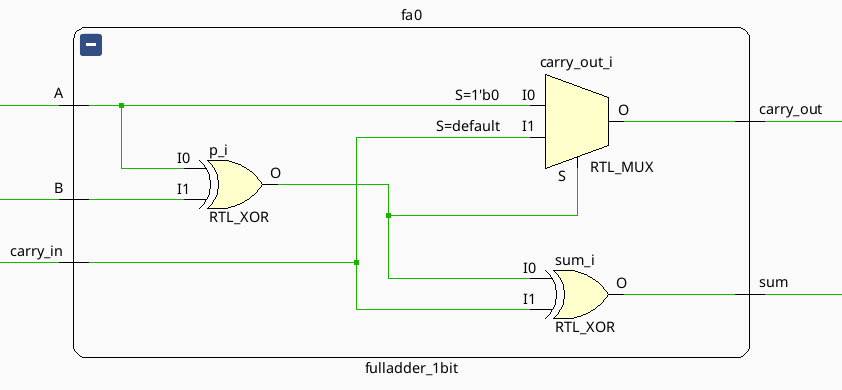
\includegraphics[width=15cm]{resources/fulladder.png}
    \caption{Circuito Logico del Full Adder}
    \label{fig:logic_circuit_fulladder}
\end{figure}

\subsection{Testbench}
Essendo presenti 3 entrate e quindi sole \(2^3=8\) possibli combinazioni, si è deciso di testare ogni caso possibile. Sono stati implementati anche gli statement \textit{assert} per verificare la correttezza degli output e quindi eseguire dei test. 

\begin{problem}{Test Full-Adder}{}
\begin{lstlisting}[language=VHDL]
library IEEE;
use IEEE.STD_LOGIC_1164.ALL;

entity testbench_fulladder is
end testbench_fulladder;

architecture Behavioral of testbench_fulladder is
  component fulladder_1bit is
    Port ( 
      A : in STD_LOGIC;
      B : in STD_LOGIC;
      carry_in : in STD_LOGIC;
      carry_out : out STD_LOGIC;
      sum : out STD_LOGIC);
    end component;
    
  signal Ia,Ib,Icin,Ocout,Osum: STD_LOGIC;
begin
  CUT: fulladder_1bit port map (Ia,Ib,Icin,Ocout,Osum);
  process begin
    --Test 1: A = 0, B = 0, carry_in = 0
    Ia <= '0'; Ib <= '0'; Icin <= '0';
    wait for 10ns;
    assert (Osum  = '0' and Ocout = '0') report "Test 1 Fallito" severity error;

    --Test 2: A = 0, B = 0, carry_in = 1
    Ia <= '0'; Ib <= '0'; Icin <= '1';
    wait for 10ns;
    assert (Osum  = '1' and Ocout = '0') report "Test 2 Fallito" severity error;
        
    --Test 3: A = 1, B = 0, carry_in = 0
    Ia <= '1'; Ib <= '0'; Icin <= '0';
    wait for 10ns;
    assert (Osum  = '1' and Ocout = '0') report "Test 3 Fallito" severity error;

    --Test 4: A = 1, B = 0, carry_in = 1
    Ia <= '1'; Ib <= '0'; Icin <= '1';
    wait for 10ns;
    assert (Osum  = '0' and Ocout = '1') report "Test 4 Fallito" severity error;

    --Test 5: A = 0, B = 1, carry_in = 0
    Ia <= '0'; Ib <= '1'; Icin <= '0';
    wait for 10ns;
    assert (Osum  = '1' and Ocout = '0') report "Test 5 Fallito" severity error;

    --Test 6: A = 0, B = 1, carry_in = 1
    Ia <= '0'; Ib <= '1'; Icin <= '1';
    wait for 10ns;
    assert (Osum  = '0' and Ocout = '1') report "Test 6 Fallito" severity error;
        
    --Test 7: A = 1, B = 1, carry_in = 0
    Ia <= '1'; Ib <= '1'; Icin <= '0';
    wait for 10ns;
    assert (Osum  = '0' and Ocout = '1') report "Test 7 Fallito" severity error;
        
    --Test 8: A = 1, B = 1, carry_in = 1 
    Ia <= '1'; Ib <= '1'; Icin <= '1';
    wait for 10ns;
    assert (Osum  = '1' and Ocout = '1') report "Test 8 Fallito" severity error;
    
  end process;
end Behavioral;
\end{lstlisting}
\end{problem}
\newpage

\subsection{Simulazione}
Il risultato della testbench sopra indicata è illustrato nella seguente simulazione:
\begin{figure}[ht]
    \center
    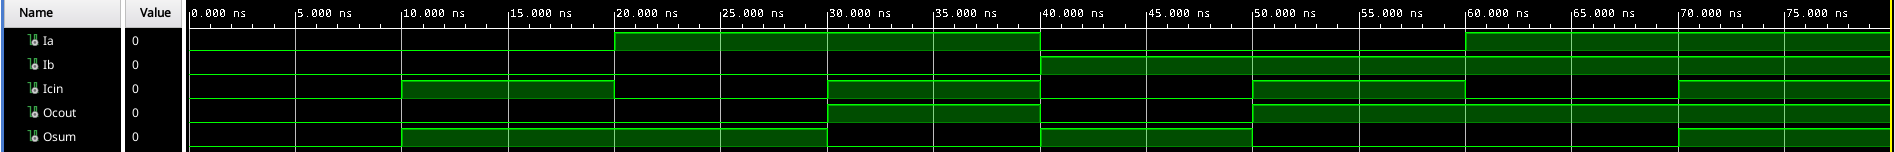
\includegraphics[width=16cm]{resources/fulladder_sim.png}
    \caption{Simulazione Full Adder}
    \label{fig:simulation_full adder}
\end{figure}

\newpage

\section{Ripple-Carry Adder a 4 bit}
\subsection{Implementazione}
L'addizionatore a propagazione del riporto conta al suo interno 4 full adder a 1 bit che lavorano insieme, il \textit{carry\_out} finale viene salvato.

\begin{problem}{Codice Ripple Carry}{}
\begin{lstlisting}[language=VHDL]
library IEEE;
use IEEE.STD_LOGIC_1164.ALL;

entity ripplecarry_4bit is
  Port ( A_4 : in STD_LOGIC_VECTOR (3 downto 0);
    B_4 : in STD_LOGIC_VECTOR (3 downto 0);
    carry_in : in STD_LOGIC;
    carry_out : out STD_LOGIC;
    sum_4 : out STD_LOGIC_VECTOR (3 downto 0));
end ripplecarry_4bit;

architecture Behavioral of ripplecarry_4bit is
  component fulladder_1bit is
    Port ( 
      A : in STD_LOGIC;
      B : in STD_LOGIC;
      carry_in : in STD_LOGIC;
      carry_out : out STD_LOGIC;
      sum : out STD_LOGIC);
  end component;
    
  signal sum, carry: STD_LOGIC_VECTOR(3 downto 0);
begin
  fa0: fulladder_1bit PORT MAP( A_4(0), B_4(0), carry_in, carry(0), sum_4(0) );
  fa1: fulladder_1bit PORT MAP( A_4(1), B_4(1), carry(0), carry(1), sum_4(1) );
  fa2: fulladder_1bit PORT MAP( A_4(2), B_4(2), carry(1), carry(2), sum_4(2) );
  fa3: fulladder_1bit PORT MAP( A_4(3), B_4(3), carry(2), carry(3), sum_4(3) );
  carry_out <= carry(3);
end Behavioral;
\end{lstlisting}
\end{problem}

\subsection{Schematica}
\begin{figure}[H]
    \centering
    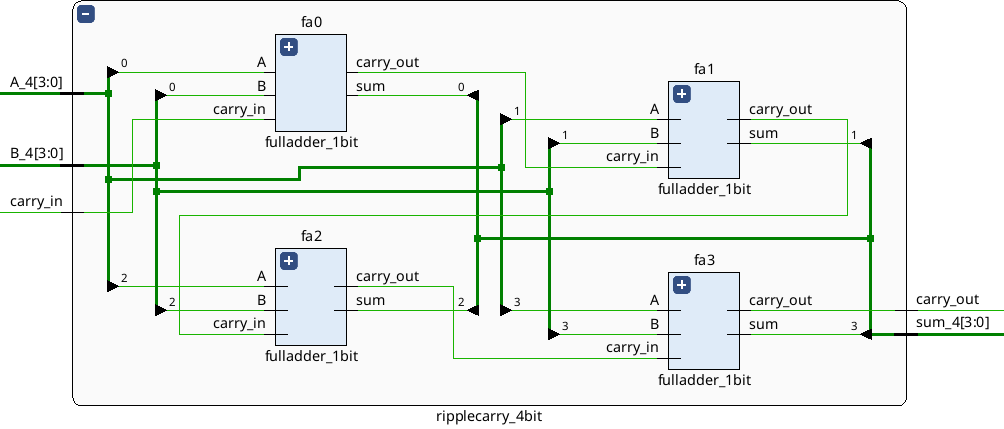
\includegraphics[width=15cm]{resources/ripplecarry.png}
    \caption{Circuito Logico del Ripple Carry Adder}
    \label{fig:logic_circuit_ripplecarry}
\end{figure}

\subsection{TestBench}
Nella fase di testing essendo impossibile testare ogni caso sono stati implementati i test soltanto di alcune situazioi notevoli.

\begin{problem}{Codice Ripple Carry}{}
\begin{lstlisting}[language=VHDL]
library IEEE;
use IEEE.STD_LOGIC_1164.ALL;

entity testbench_ripplecarry is
end testbench_ripplecarry;

architecture Behavioral of testbench_ripplecarry is
  component ripplecarry_4bit is
    Port ( 
    A_4 : in STD_LOGIC_VECTOR (3 downto 0);
    B_4 : in STD_LOGIC_VECTOR (3 downto 0);
    carry_in : in STD_LOGIC;
    carry_out : out STD_LOGIC;
    sum_4 : out STD_LOGIC_VECTOR (3 downto 0));
  end component;

  signal Ia,Ib,Osum: std_logic_vector (3 downto 0);
  signal Icin,Ocout:std_logic;
  
begin
  CUT: ripplecarry_4bit port map (Ia,Ib,Icin,Ocout ,Osum);
  process begin
    --Test 1: caso base, A = 0, B = 0, carry = 0
    Ia <= "0000"; Ib <= "0000"; Icin <= '0';
    wait for 10ns;
    assert ( Osum = "0000" and Ocout = '0') report "Test case 1 Failed" severity error;

    --Test 2: A = 1, B = 1, carry = 0
    Ia <= "0001"; Ib <= "0001"; Icin <= '0';
    wait for 10ns;
    assert ( Osum = "0010" and Ocout = '0') report "Test case 2 Failed" severity error;

    --Test case 3: A = 0101, B = 0011, carry_in = 0
    Ia <= "0101"; Ib <= "0011"; Icin <= '0';
    wait for 10 ns;
    assert (Osum = "1000" and Ocout= '0') report "Test case 3 failed";

    -- Test case 4: A = 1111, B = 0001, carry_in = 0
    Ia <= "1111"; Ib <= "0001"; Icin <= '0';
    wait for 10 ns;
    assert (Osum = "0000" and Ocout = '1') report "Test case 4 failed" severity error;

    -- Test case 5: Ia = 1111, Ib = 1111, cin = 0
    Ia <= "1111"; Ib <= "1111"; Icin <= '0';
    wait for 10 ns;
    assert (Osum = "1110" and Ocout = '1') report "Test case 5 failed" severity error;

    -- Test case 6: Ia = 1010, Ib = 0101, cin = 1
    Ia <= "1010"; Ib <= "0101"; Icin <= '1';
    wait for 10 ns;
    assert (Osum = "0000" and Ocout = '1') report "Test case 6 failed" severity error;

    -- Test case 7: Ia = 1001, Ib = 1001, cin = 0
    Ia <= "1001"; Ib <= "1001"; Icin <= '0';
    wait for 10 ns;
    assert (Osum = "0010" and Ocout = '1') report "Test case 7 failed" severity error;

    -- Test case 8: Ia = 0110, Ib = 1001, cin = 1
    Ia <= "0110"; Ib <= "1001"; Icin <= '1';
    wait for 10 ns;
    assert (Osum = "0000" and Ocout = '1') report "Test case 8 failed" severity error;
    
    end process;
end Behavioral;

\end{lstlisting}
\end{problem}

\subsection{Simulazione}
Il risultato della testbench sopra indicata è illustrato nella seguente simulazione:
\begin{figure}[h]
    \centering
    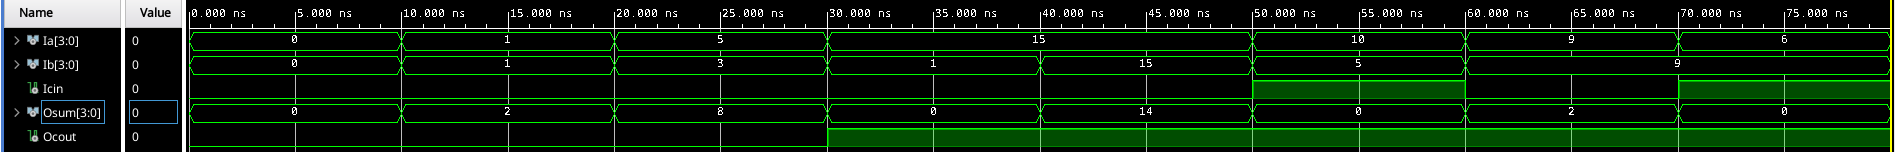
\includegraphics[width=16cm]{resources/ripple_carry_sim.png}
    \caption{Simulazione Ripple Carry}
    \label{fig:simulation_ripple_carry}
\end{figure}



\newpage

\section{Carry-Select Adder}
\subsection{Implementazione}
Nella fase iniziale vengono istanziati i vari addizionatori Ripple Carry con le loro varianti con \textit{carry\_in} '0' e '1', con il costrutto \textit{when else} viene selezionato quale risultato delle somme è quello da utilizzare, la variabile che ha il ruolo di selezionatore è \textit{carry\_selector} che è assegnata al valore del riporto dell'addizionatore precedente, è una variabile shared perché deve essere acceduta in più di un processo. Si è optato per una assegnazione di tipo dichiarativa piuttosto che posizionale, producendo un codice più lungo ma anche più robusto.
Per il risultato si è deciso di utilizzare un vettore di \textit{STD\_LOGIC} a 17 bit piuttosto che a 16 allo scopo di prevenire l'overflow.

\begin{problem}{Codice Carry Select}{}
\begin{lstlisting}[language=VHDL]
library IEEE;
use IEEE.STD_LOGIC_1164.ALL;

entity carry_select_16bit is
  Port ( 
    A : in STD_LOGIC_VECTOR (15 downto 0);
    B : in STD_LOGIC_VECTOR (15 downto 0);
    carry_in_start: in STD_LOGIC;
    sum : out STD_LOGIC_VECTOR (16 downto 0);
end carry_select_16bit;

architecture Behavioral of carry_select_16bit is

  component ripplecarry_4bit is
    Port (
      A_4 : in STD_LOGIC_VECTOR (3 downto 0);
      B_4 : in STD_LOGIC_VECTOR (3 downto 0);
      carry_in : in STD_LOGIC;
      carry_out : out STD_LOGIC;
      sum_4 : out STD_LOGIC_VECTOR (3 downto 0));
  end component;

  shared variable carry_selector: STD_LOGIC;
  signal carry_start: STD_LOGIC;
  signal carry0, carry1: STD_LOGIC_VECTOR(2 downto 0);
  signal sum_0, sum_1: STD_LOGIC_VECTOR(12 downto 0);
    
begin
  ripplecarry0_0: ripplecarry_4bit PORT MAP (
    A_4 => A(3 downto 0),
    B_4 => B(3 downto 0),
    carry_in => carry_in_start,
    carry_out => carry_start,
    sum_4 => sum(3 downto 0));

  ripplecarry1_0: ripplecarry_4bit PORT MAP (
    A_4 => A(7 downto 4),
    B_4 => B(7 downto 4),
    carry_in => '0',
    carry_out => carry0(0),
    sum_4 => sum_0(3 downto 0));
  ripplecarry1_1: ripplecarry_4bit PORT MAP (
    A_4 => A(7 downto 4),
    B_4 => B(7 downto 4),
    carry_in => '1',
    carry_out => carry1(0),
    sum_4 => sum_1(3 downto 0));

  ripplecarry2_0: ripplecarry_4bit PORT MAP (
    A_4 => A(11 downto 8),
    B_4 => B(11 downto 8),
    carry_in => '0',
    carry_out => carry0(1),
    sum_4 => sum_0(7 downto 4));
  ripplecarry2_1: ripplecarry_4bit PORT MAP (
    A_4 => A(7 downto 4),
    B_4 => B(7 downto 4),
    carry_in => '1',
    carry_out => carry1(1),
    sum_4 => sum_1(7 downto 4));

  ripplecarry3_0: ripplecarry_4bit PORT MAP (
    A_4 => A(15 downto 12),
    B_4 => B(15 downto 12),
    carry_in => '0',
    carry_out => carry0(2),
    sum_4 => sum_0(11 downto 8));
  ripplecarry3_1: ripplecarry_4bit PORT MAP (
    A_4 => A(15 downto 12),
    B_4 => B(15 downto 12),
    carry_in => '1',
    carry_out => carry1(2),
    sum_4 => sum_1(11 downto 8));
   
  process(carry_start, sum_0, sum_1, carry_start) begin
    case carry_start is
      when '0' =>
        sum( 7 downto 4 ) <= sum_0(3 downto 0);
        carry_selector := carry0(0);
      when  others =>
        sum( 7 downto 4 ) <= sum_1(3 downto 0);
        carry_selector := carry1(0);
    end case;

    case carry_selector is
      when '0' =>
        sum( 11 downto 8 ) <= sum_0(7 downto 4);
        carry_selector := carry0(1);
      when  others =>
        sum( 11 downto 8 ) <= sum_1(7 downto 4);
        carry_selector := carry1(1);
    end case;

    case carry_selector is
      when '0' =>
        sum( 15 downto 12 ) <= sum_0(11 downto 8);
        carry_selector := carry0(2);
      when  others =>
        sum( 15 downto 12 ) <= sum_1(11 downto 8);
        carry_selector := carry1(2);
    end case;
      sum(16) <= carry_selector;
  end process;
end Behavioral;
\end{lstlisting}
\end{problem}
\subsection{Schematica}
La schematica del carry select adder comprende 7 ripplecarry adder a 4 bit e 6 multiplexer.
Degno di nota è che nel codice non è presente alcun multiplexer, questi vengono infatti generati automaticamente a partire dalle istruzioni condizionali.
\begin{figure}[H]
    \centering
    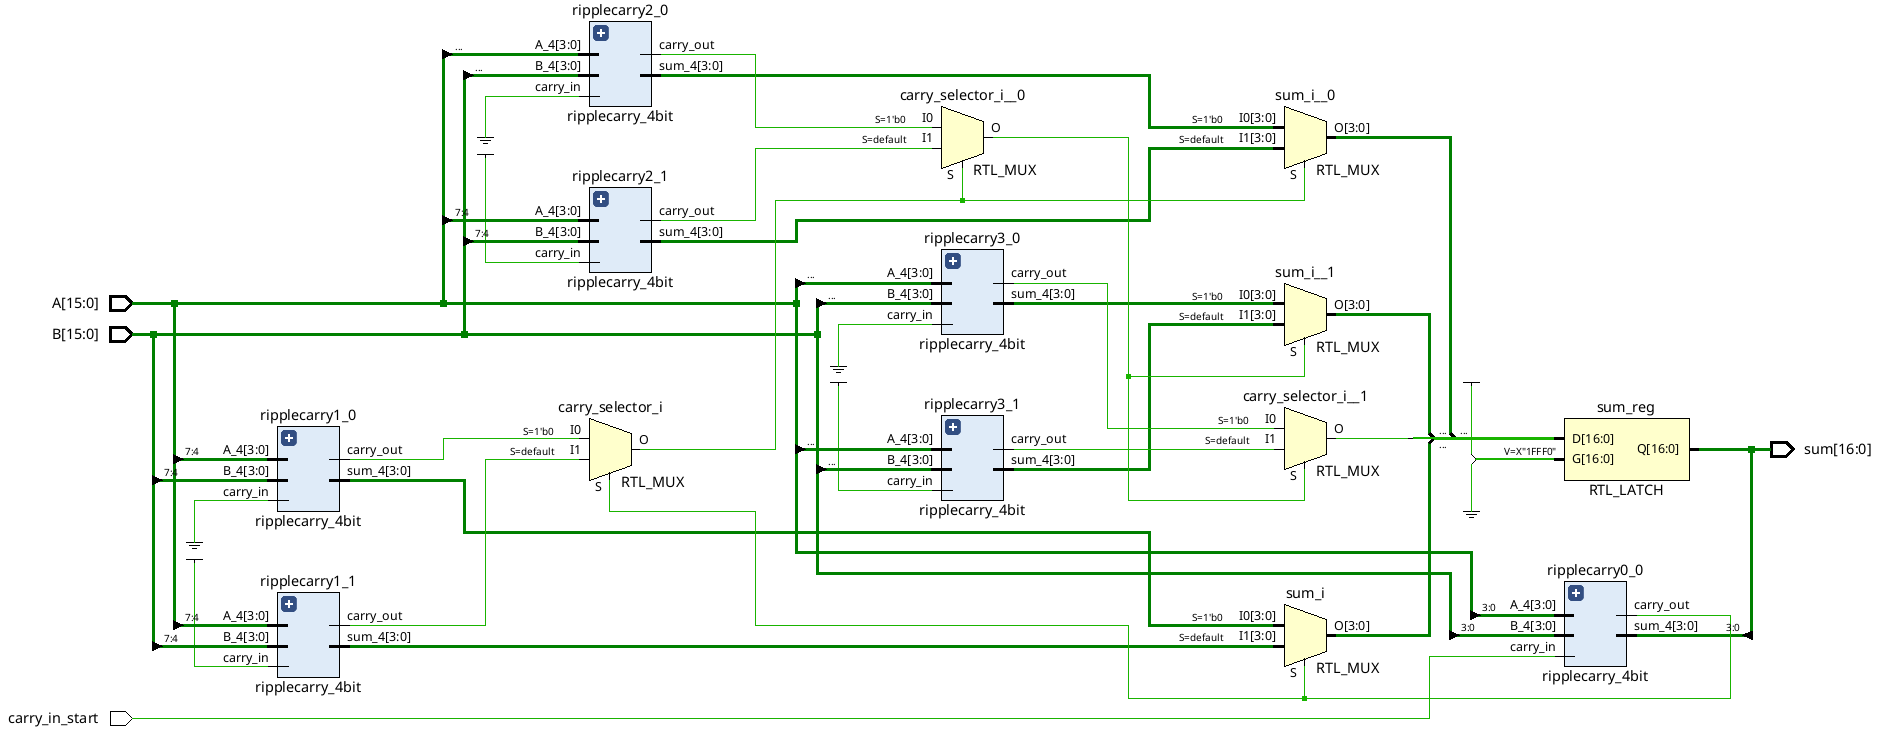
\includegraphics[width=15cm]{resources/carry_select_schematics.png}
    \caption{Circuito Logico del Carry Select Adder}
    \label{fig:logic_circuit_carry_select_adder}
\end{figure}
\subsection{Testbench}
Discorso analogo a quello del Ripple Carry Adder.
\begin{problem}{Codice Carry Select}{}
\begin{lstlisting}[language=VHDL]
library IEEE;
use IEEE.STD_LOGIC_1164.ALL;

entity testbench_carryselect is
end testbench_carryselect;

architecture Behavioral of testbench_carryselect is
  component carry_select_16bit is
    Port ( 
      A : in STD_LOGIC_VECTOR (15 downto 0);
      B : in STD_LOGIC_VECTOR (15 downto 0);
      carry_in_start: in STD_LOGIC;
      sum : out STD_LOGIC_VECTOR (16 downto 0));
  end component;
  signal Ia,Ib: STD_LOGIC_VECTOR (15 downto 0);
  signal Os: STD_LOGIC_VECTOR (16 downto 0);
  signal Icin: STD_LOGIC;
begin
  CUT: carry_select_16bit port map(Ia,Ib,Icin,Os);
    
  process begin    
    -- Test 1: A = 0000000000000000, B = 0000000000000000, carry_in = 0
    Ia <= (others => '0'); 
    Ib <= (others => '0'); 
    Icin <= '0';
    wait for 10 ns;
    assert (Os = "00000000000000000")
    report "Test 1 Fallito: La somma di zero deve essere zero." severity error;

    -- Test 2: A = 0000000000000000, B = 0000000000000000, carry_in = 1
    Ia <= (others => '0'); 
    Ib <= (others => '0'); 
    Icin <= '1';
    wait for 10 ns;
    assert (Os = "00000000000000001") 
    report "Test 2 Fallito: La somma di zero e riporto deve essere uno." severity error;

    -- Test 3: A = 0111111111111111, B = 0000000000000001, carry_in = 0
    Ia <= "0111111111111111";  -- 32767
    Ib <= "0000000000000001";  -- 1
    Icin <= '0';
    wait for 10 ns;
    assert (Os = "10000000000000000") 
    report "Test 3 Fallito: Somma deve essere 32768 (overflow positivo)." severity error;

    -- Test 4: A = 0111111111111111, B = 0111111111111111, carry_in = 0
    Ia <= "0111111111111111";  -- 32767
    Ib <= "0111111111111111";  -- 32767
    Icin <= '0';
    wait for 10 ns;
    assert (Os = "11111111111111110") 
    report "Test 4 Fallito: Somma deve essere 65534 (overflow positivo)." severity error;

    -- Test 5: A = 0000000000000001, B = 0000000000000001, carry_in = 1
    Ia <= "0000000000000001";  -- 1
    Ib <= "0000000000000001";  -- 1
    Icin <= '1';
    wait for 10 ns;
    assert (Os = "00000000000000011") report "Test 5 Fallito: Somma deve essere 3 con riporto." severity error;

    -- Test 6: A = 0000000000000000, B = 1111111111111111, carry_in = 0
    Ia <= "0000000000000000"; 
    Ib <= "1111111111111111";  -- 65535
    Icin <= '0';
    wait for 10 ns;
    assert (Os = "01111111111111111") report "Test 6 Fallito: Somma deve essere 65535." severity error;

    -- Test 7: A = 1111111111111111, B = 1111111111111111, carry_in = 1
    Ia <= "1111111111111111";  -- 65535
    Ib <= "1111111111111111";  -- 65535
    Icin <= '1';
    wait for 10 ns;
    assert (Os = "11111111111111110") 
    report "Test 7 Fallito: Somma deve essere 65535 con overflow e riporto." severity error;

    -- Test 8: A = 1111111111111111, B = 0000000000000001, carry_in = 0
    Ia <= "1111111111111111";  -- 65535
    Ib <= "0000000000000001";  -- 1
    Icin <= '0';
    wait for 10 ns;
    assert (Os = "10000000000000000") report "Test 8 Fallito: Somma deve essere 0 (overflow)." severity error;

    --Test Finiti
    report "Tutti i test sono stati completati con successo!" severity note;
  end process;
end Behavioral;
\end{lstlisting}
\end{problem}
\subsection{Simulazione}
Il risultato della testbench sopra indicata è illustrato nella seguente simulazione:
\begin{figure}[h]
    \centering
    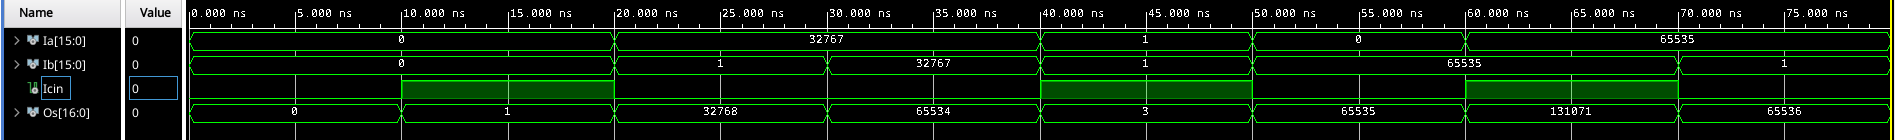
\includegraphics[width=16cm]{resources/carry_select_sim.png}
    \caption{Simulazione Carry Select}
    \label{fig:simulation_carryselect}
\end{figure}
\end{document}
